\documentclass[a4paper, 12pt]{article}

\usepackage[portuguese]{babel}
\usepackage[utf8]{inputenc}
\usepackage[T1]{fontenc}
\usepackage{array}
\usepackage{fixltx2e}
\usepackage{amsmath}
\usepackage{amssymb}
\usepackage{graphicx}
\usepackage{caption}
\usepackage{float}
\usepackage{a4wide}
\usepackage{multicol}
\usepackage[table]{xcolor}
\usepackage{makeidx}
\usepackage{hyperref}
\usepackage{setspace}
\usepackage{indentfirst}
\usepackage[nottoc]{tocbibind}
\usepackage{listings}
\usepackage[font=footnotesize,labelfont=bf]{caption}
\usepackage[a4paper,top=1.60cm,bottom=1.60cm,left=1.37cm,right=1.45cm]{geometry}
\usepackage[square, sort, comma, numbers]{natbib}

\onehalfspacing
\graphicspath{{./img/}}
\makeindex

\usepackage{tikz}
\usetikzlibrary{calc,trees,positioning,arrows,chains,shapes.geometric,%
    decorations.pathreplacing,decorations.pathmorphing,shapes,%
    matrix,shapes.symbols}

\tikzset{
>=stealth',
  punktchain/.style={
    rectangle,
    rounded corners,
    draw=black, very thick,
    text width=8.3em,
    minimum height=1em,
    text centered,
    on chain},
  fillchain/.style={
    rectangle,
    rounded corners,
    fill=blue!30,
    draw=black, very thick,
    text width=8.3em,
    minimum height=1em,
    text centered,
    on chain},
  line/.style={draw, thick, <-},
  element/.style={
    tape,
    top color=white,
    bottom color=blue!50!black!60!,
    minimum width=4em,
    draw=blue!40!black!90, very thick,
    text width=8.3em,
    minimum height=1.5em,
    text centered,
    on chain},
  every join/.style={->, thick,shorten >=1pt},
  decoration={brace},
  tuborg/.style={decorate},
  tubnode/.style={midway, right=2pt},
}

\lstset{
    basicstyle=\footnotesize,
    morekeywords={either,or,transform,rule,to,from,through,function},
    frame=L,
}

\setcounter{secnumdepth}{2}
\setcounter{tocdepth}{2}

\begin{document}

\hypersetup{backref,pdfpagemode=FullScreen,colorlinks=true}

\thispagestyle{empty}
\begin{center}
    \vspace*{4cm}
    \textbf{\Large{Resolução Automatizada de Problemas Difíceis \\ em Ambientes Heterogêneos: \\ Uma Abordagem baseada em \\ Combinação, Sintonia Fina e Adaptação}}\\

    \vskip 1cm

    \textsc{Projeto de Pesquisa para Doutorado Direto}

    \vskip 3cm

    \begin{minipage}{.4\linewidth}
        \begin{flushleft}
            \emph{Autor}: \\Pedro \textsc{Bruel}\\
            pedro.bruel@gmail.com
        \end{flushleft}
    \end{minipage}
    \begin{minipage}{.4\linewidth}
        \begin{flushright}
            \emph{Orientador}: \\Prof. Dr. Alfredo \textsc{Goldman}\\
            gold@ime.usp.br
        \end{flushright}
    \end{minipage}

    \vskip 1cm

    \normalsize{\emph{DCC - IME\\
    Universidade de São Paulo}\\}

    % Correct Line width for this document:
    %\begin{abstract}
    %\rule{\linewidth}{.1mm} \\
    %\rule{\linewidth}{.1mm} \\
    %\end{abstract}

    \vfill
    \normalsize{São Paulo, \today}
\end{center}

\newpage

\abstract
\noindent
\rule{\linewidth}{.1mm} \\
\noindent
A grande variedade de arquiteturas de computador torna o desenvolvimento e a
otimização de programas eficientes um esforço que deve ser repetido para cada
nova arquitetura em que se pretenda atingir um bom desempenho.
Trabalhos na área da otimização automática de programas utilizam métodos
empíricos para realizar uma busca por escolhas de implementação e compilação.
Auxiliados pela crescente disponibilidade de ciclos computacionais,
buscam encontrar escolhas que otimizem o desempenho da solução de um problema
em diferentes arquiteturas de computador. Os objetivos deste projeto de
pesquisa relacionam-se ao estudo das possibilidades das estratégias para
Multi-Seleção e execução em algoritmo \emph{portfolio} implementadas no sistema
AMF e seu uso como técnicas de \emph{auto-tuning}.
Essas estratégias serão implementadas como componentes dos sistemas PetaBricks
e OpenTuner, para a resolução de casos que envolvam problemas de decisão
computacionalmente difíceis.
Serão também adaptadas à solução do problema do \emph{auto-tuning online} e ao
\emph{auto-tuning} de problemas de otimização.
O desempenho das estratégias implementadas será medido em arquiteturas
computacionais variadas e analisado através de um conjunto de
\emph{benchmarks}. As estratégias implementadas devem permitir a especificação
dos espaços de soluções de um mesmo problema e a otimização automática da
solução de instâncias desse problema em uma dada arquitetura.

\noindent
\rule{\linewidth}{.1mm} \\

\tableofcontents

\newpage

\section{Introdução} \label{sec:intro}

Recentes avanços na construção de arquiteturas de computador, como
por exemplo processadores com múltiplos núcleos e novas arquiteturas
e métodos de acesso a memória, criam novas possibilidades para o
desenvolvimento de aplicações paralelas. Somando-se a esses avanços, o contínuo
barateamento e o aumento da disponibilidade de ciclos de processamento incitam
a exploração de métodos empíricos e automáticos para a otimização de programas,
em busca da portabilidade não só de execução, mas também de desempenho.

Encontram-se na literatura diversos de métodos e ferramentas para otimização
automática de código que visam minimizar o esforço associado ao desenvolvimento
e manutenção de código portável, funcional e eficiente. Motivados pela grande
variedade e rápida mudança das arquiteturas de computador atuais, esses
trabalhos procuram explorar de forma mais completa o paralelismo inerente às
novas arquiteturas computacionais. Esse potencial paralelismo é proveniente de
diversas características, como por exemplo múltiplos núcleos de processamento,
diferentes arquiteturas de memória distribuída, compartilhada (de acesso
uniforme, não uniforme) e auxílio de coprocessadores.

A estratégia para a otimização automática de um programa pode envolver
modelagens da arquitetura alvo, o que exige conhecimentos específicos sobre o
problema e a máquina em questão. Por outro lado, podem ser utilizadas técnicas
de aprendizado de máquina para realizar buscas empíricas no espaço de possíveis
soluções de um problema, encontrando a melhor otimização através de medidas de
desempenho numa dada arquitetura de computador.

Dentre os trabalhos que implementam estratégias de otimização automática
baseadas no processo de busca empírica, alguns compiladores realizam uma
calibragem dos parâmetros de compilação (\citet{bilmes1997,whaley1998}) para a
arquitetura alvo e utilizam essa calibragem para gerar código otimizado para
essa arquitetura. Este processo é feito uma única vez em tempo de instalação
do sistema e deve ser repetido em cada nova arquitetura.

Outros trabalhos (\citet{goldman2012framework,mitcsail-tr:2014,
vuduc2004}) propõe uma abordagem diferente, que envolve gerar e executar
combinações algorítmicas para a solução de um mesmo problema. A melhor
combinação é então selecionada empiricamente através da técnica de busca
implementada pelo trabalho.

Os enormes espaços de busca resultantes da combinação das diferentes formas de
se implementar um algoritmo para solução de um determinado problema motivam
a pesquisa e o desenvolvimento de técnicas empíricas de busca. Outros fatores
também compõe essa motivação, como a dificuldade de se modelar o impacto no
desempenho de pequenas variações na implementação dos algoritmos e a grande
quantidade de variáveis de arquitetura e de ambiente envolvidas na execução de
um programa.

A seguir será feita uma exposição do problema da otimização automática
(Seção \ref{sec:auto-tuning}), que contextualizará uma discussão das
estratégias para otimização implementadas pelos sistemas
OpenTuner (Seção \ref{sec:opent}), PetaBricks (Seção \ref{sec:peta}) e AMF
(Seção \ref{sec:amf}). O objetivo deste projeto de pesquisa é explorar as
possibilidades das técnicas para cálculo e execução de algoritmos
\emph{portfolio}, implementadas no AMF, no desenvolvimento de soluções para o
problema da otimização automática, no contexto de diferentes arquiteturas
computacionais.

O restante deste projeto está organizado da seguinte forma:
A Seção \ref{sec:trabrel} apresenta um levantamento bibliográfico com breves
discussões sobre os principais trabalhos relacionados à proposta.
A Seção \ref{sec:obj} detalha os objetivos do projeto. Na Seção
\ref{sec:met}, discute-se a metodologia de desenvolvimento e avaliação de
resultados. Finalmente, a Seção \ref{sec:sched} apresenta um plano de trabalho
e um cronograma para seu desenvolvimento.

\subsection{Auto-tuning} \label{sec:auto-tuning}

Ao desenvolver uma solução portável e eficiente para um problema, o
programador deve considerar, entre outros fatores, as possibilidades
de implementação dos algoritmos que resolvem o problema e as otimizações e
parâmetros disponibilizados pelo compilador.
A escolha da melhor implementação de um algoritmo e do melhor conjunto de
valores para parâmetros de compilação depende em grande parte das arquiteturas
e ambientes em que se pretende executar o programa. O programador realizará
as escolhas de implementação baseando-se em seus conhecimentos das arquiteturas
alvo e resultados de testes que realiza durante o desenvolvimento.

No entanto, as arquiteturas de computador atuais variam muito, num grande
espectro de, por exemplo, tamanhos de \emph{RAM},
velocidades e modos de acesso a níveis de memória e armazenamento, número de
núcleos no processador e coprocessadores --- \emph{GPU}s, entre outros
--- que apresentam ainda sua própria gama de variação. Essa variação é
ainda maior se considerarmos as arquiteturas de memória com acesso
não uniforme.

Devido a essa heterogeneidade e sua rápida taxa de mudança,
o trabalho de produzir implementações portáveis e eficientes
dependerá cada vez mais de conhecimentos específicos sobre uma arquitetura,
motivando o desenvolvimento de técnicas automáticas de seleção das melhores
implementações para solução de um problema, isto é, o \emph{auto-tuning} de um
conjunto de soluções possíveis.

Como exemplo para a seleção de implementações diferentes para um mesmo
problema, considere a multiplicação de matrizes. O melhor algoritmo
para multiplicação de duas matrizes depende, por exemplo, do tamanho dessas
matrizes, do tempo de acesso e tamanho de \textit{cache} do processador e das
possibilidades para exploração do paralelismo da arquitetura.
Para ilustrar a seleção de valores para parâmetros de compilação, considere
a escolha de opções, ou \emph{flags}, de compilação.
~\citet{tartara2013heuristics} apresentam um algoritmo para seleção de
heurísticas de compilação e utilizam a seleção de \emph{flags}
do GCC para demonstrar o algoritmo, implementado em extensões do PetaBricks e
do próprio GCC.
O alto número de \emph{flags} disponíveis numa dada arquitetura e as interações
complexas entre as diferentes opções fazem do conjunto dos problemas de
seleção do melhor algoritmo para multiplicação de matrizes e de seleção de
\emph{flags} de compilador, um bom candidato para solução por
\emph{auto-tuning}.

\subsubsection{Descrição do Problema}

O problema do \emph{auto-tuning}, através do processo de escolha algorítmica,
pode ser descrito da seguinte forma (\citet{ansel2011efficient}):

Considere o conjunto $A$ de algoritmos que resolvem instâncias de um dado
problema, o conjunto $S$ de seletores para esses algoritmos e o conjunto $S_t$
de seletores para parâmetros de compilação e configuração no conjunto $B$.
O seletor $s \in S$ de algoritmos em $A$ consiste em
$\overrightarrow{C_s} = [c_{s,1},\dots,c_{s,m-1}] \cup \overrightarrow{A_s} =
[\alpha_{s,1},\dots,\alpha_{s,m-1}]$,
onde cada $c_{s,i} \in \overrightarrow{C_s}$ representa um intervalo
relacionado a um tamanho de entrada para a instância e
determina a execução do algoritmo $\alpha_{s,i} \in \overrightarrow{A_s},
\quad \alpha_{s,i} \in A$ neste intervalo.
Além disso, $min(n) \leq c_{s,1} < n < c_{s,m-1} \leq max(n)$,
onde $n$ é o tamanho da entrada para a instância sendo selecionada e $m$
é determinado pela instância.
Assim, um seletor $s \in S$ seleciona algoritmos da seguinte forma:

\begin{equation*}
    SELECT(s, i) = \alpha_{s,i} \in \overrightarrow{A_{s}} \quad | \quad c_{s,i} \in \overrightarrow{C_{s}},
    \quad\quad 1 \leq i < m
\end{equation*}

Além de um seletor para algoritmos, podemos especificar seletores $s_t \in S_t$,
compostos de $\overrightarrow{B_{s_t}} = [\beta_{s_t,1},\dots,\beta_{s_t,b-1}]
\cup \overrightarrow{V_{s_t}} = [v_{s_t,1},\dots,v_{s_t,b-1}]$,
onde cada $\beta_{s_t,j} \in \overrightarrow{B_{s_t}}$ representa um parâmetro
de compilação ou configuração para a instância do problema, que assume o valor
especificado por $v_{s_t,i} \in \overrightarrow{V_{s_t}}$.
O seletor $s_t$ seleciona um valor para cada parâmetro de compilação e
configuração definido para a instância:

\begin{equation*}
    SELECT_{\beta}(s_t, j) = v_{s_t,j} \in \overrightarrow{V_{s_t}} \quad | \quad \beta_{s_t,j} \in \overrightarrow{B_{s_t}},
    \quad\quad 1 \leq j < b
\end{equation*}

Com os seletores $s$ e $s_t$, podemos especificar um programa
$P_{s,s_t}$ e o objetivo de um \emph{auto-tuner} ideal é encontrar
os seletores $s^*,s_{t}^{*}$ que especifiquem o programa $P_{s^*,s_{t}^{*}}$,
ou $P^*$, cujo tempo de execução $t^*$ --- representado por $T(P^*,H,n)$ ---
é calculado executando-se o programa na arquitetura $H$, com entrada de tamanho
$n$ e deve satisfazer:

\begin{equation*}
    t^* = T(P^*,H,n) \leq T(P_{s^*,s_{t}^{*}},H,n), \quad \forall s \in S, \quad \forall s_t \in S_t
\end{equation*}

\subsubsection{Algumas Características do Problema}

Em problemas computacionalmente fáceis, o tempo de execução dos programas
especificados pelos seletores será polinomialmente proporcional ao tamanho da
entrada, facilitando o uso de testes empíricos para determinar as melhores
combinações algorítmicas. Problemas computacionalmente difíceis, por outro
lado, precisam ser abordados de forma diferente --- através de, por exemplo,
aproximações e heurísticas --- cujo tempo de execução pode depender de
diferentes características da entrada. Isso sugere que o melhor método de busca
no espaço de soluções para problemas computacionalmente difíceis será diferente
daquele para o caso de problemas computacionalmente fáceis.

O tempo de execução dos programas especificados pelos seletores também sofre
interferência de muitos outros fatores, como por exemplo outros processos
executados pelo sistema operacional competindo por recursos computacionais.
As propriedades da avaliação do desempenho de soluções para diferentes classes
de problema contribuirão para o desenvolvimento e a escolha dos métodos
que serão utilizados no \emph{auto-tuner}.

No restante da Seção \ref{sec:intro}, serão discutidos os algoritmos, técnicas
e estratégias utilizadas por alguns sistemas na solução de problemas de
\emph{auto-tuning}. Na Seção \ref{sec:opent}, é discutido o OpenTuner,
um arcabouço cujo objetivo é permitir a especificação de \emph{auto-tuners}
para diferentes domínios de problema. Na Seção \ref{sec:auto-tuner}, é discutido
o sistema PetaBricks e sua implementação de um algoritmo genético para realizar
o \emph{auto-tuning}. Na Seção \ref{sec:multsel}, discute-se as estratégias
utilizadas pelo sistema AMF, que se baseiam em cálculos de distribuição de
recursos computacionais e execução em \emph{portfolio}.

\subsection{OpenTuner} \label{sec:opent}

As técnicas de \emph{auto-tuning} geram programas com desempenho melhor e
muitas vezes portável, podendo atingir desempenho semelhante em diferentes
arquiteturas (\citet{demmel2009accelerating}). Por outro lado, cada
implementação dessas técnicas é altamente especializada para um problema
específico, como por exemplo multiplicação de matrizes ou cálculos de
processamento de sinais digitais.
O OpenTuner (\citet{ansel2013opentuner}) é um arcabouço para a geração de
\emph{auto-tuners} para diferentes domínios de problemas, que trata o problema
do \emph{auto-tuning} como um problema de busca e utiliza um conjunto de
técnicas de busca para realizar a otimização, executadas em paralelo.

Para implementar um \emph{auto-tuner} através do OpenTuner, deve-se representar
o domínio do problema a ser otimizado na forma de um espaço de busca, definido
por um conjunto de variáveis e seus limites permitidos. As técnicas de busca
utilizadas na otimização podem ser escolhidas pela aplicação e novas técnicas
podem ser implementadas. O OpenTuner utiliza uma técnica para a
distribuição dos recursos computacionais disponíveis entre as
diversas técnicas de busca implementadas, chamada de metatécnica.
Simplificadamente, quanto melhores os resultados encontrados por uma técnica de
busca, mais recursos computacionais são disponibilizados a ela pela
metatécnica. Assim como as técnicas de busca, novas metatécnicas podem ser
implementadas para cada aplicação.

Dentre as técnicas de busca já disponíveis no OpenTuner estão a busca
aleatória, a evolução diferencial e o método Nelder-Mead. Esse conjunto
de técnicas, chamado de \emph{ensemble}, pretende ter bom desempenho em espaços
de busca bem variados e pode ser ajustado para cada aplicação. Por padrão, o
OpenTuner utiliza uma adaptação da técnica MAB AUC (\emph{Multi Armed Bandit
with sliding window, Area Under the Curve credit assignment}), como apresentada
em \citet{pacula2012bandit}, como metatécnica para distribuição de recursos
computacionais entre as técnicas de um \emph{ensemble}.

\subsubsection{MAB AUC}

A técnica de cálculo de distribuição de recursos computacionais utilizada
pelo OpenTuner tem como objetivo balancear a descoberta de novas técnicas
de busca que dão bons resultados e a exploração de técnicas cujo desempenho
já é conhecidamente bom (\emph{exploitation vs. exploration}). Na decisão sobre
qual a parcela de recursos computacionais destinada a uma técnica $t$, por
exemplo, o algoritmo MAB AUC analisa uma parcela do histórico de desempenho
dessa técnica, representado pela área sobre uma curva, desenhada durante a
execução dos testes. Caso a técnica encontre uma solução com desempenho melhor
do que o desempenho atual, a parcela de sua curva de desempenho relacionada a
esse instante será desenhada de forma crescente. Caso não encontre uma solução
melhor do que a atual, é desenhada uma linha paralela ao eixo horizontal. A
área total da curva de desempenho de uma técnica --- dentro de uma janela de
análise -- é então normalizada e representa a quantidade de crédito que a
técnica receberá na distribuição de recursos computacionais. O cálculo desse
crédito no OpenTuner, para uma técnica $t$ com curva de desempenho $V_t$, pode
ser escrito:

\begin{equation*}
    AUC_t = \frac{2} {|V_t|(|V_t|+1)} \sum_{i=1}^{|V_t|} iV_{t,i}
\end{equation*}

Onde $V_{t,i} = 1$ caso a solução encontrada pela técnica $t$ no instante
$i$ teve desempenho melhor que a melhor técnica nesse instante e
$V_{t,i} = 0$ caso contrário. O resultado de $AUC_t$ é então utilizado para
determinar qual técnica de busca será utilizada para realizar a busca atual.
A técnica $t$ que maximizar o MAB AUC realizará o teste atual. O MAB AUC é
representado por:

\begin{equation*}
    max \left( AUC_t + C\sqrt{\frac{2log|H|}{H_t}} \right)
\end{equation*}

Onde $C$ é o termo responsável por controlar o balanço entre a exploração de
uma técnica conhecida e a descoberta dos resultados de novas técnicas, $|H|$ é
o tamanho da janela de análise e $H_t$ é o número de vezes em que a técnica $t$
foi aplicada durante a janela.

\subsection{PetaBricks} \label{sec:peta}

O sistema PetaBricks (\citet{ansel2009petabricks, ansel2014phd,
ansel:xrds:2010, mitcsail-tr:2014})
consiste em uma linguagem, um compilador e um ambiente de execução,
e seu objetivo é encontrar uma sequência de aplicação de algoritmos
para a solução de um mesmo problema que especifique um programa com o melhor
desempenho na arquitetura alvo, através de uma busca empírica num espaço
de soluções definido pelo programador.

A linguagem PetaBricks (\emph{.pbcc}) facilita a
elaboração do espaço de busca pelo programador, que pode expor ao compilador
--- através de construções de alto nível --- as escolhas algorítmicas
para solução de um problema e suas ordens de execução válidas. O programa é
compilado para a linguagem C++ e então passa pelo \emph{auto-tuner}
(\citet{ansel2011efficient}), que utiliza um algoritmo genético para gerar e
testar diferentes combinações, produzindo uma configuração otimizada para
execução na arquitetura alvo.

\subsubsection{Linguagem}

A linguagem do sistema PetaBricks não possui mecanismos para controle do fluxo
de execução do programa. É possível especificar apenas modos de solução e
condições de parada e o fluxo de execução entre esses modos será determinado
pelo processo de otimização.
Tomando como exemplo o problema da ordenação de vetores, um programa no
PetaBricks pode utilizar a primitiva \emph{either...or}
(Figura~\ref{fig:sort2pbcc}) ou os conceitos de \emph{transform} e \emph{rule}
(Figura~\ref{fig:sortpbcc}) para determinar o espaço de algoritmos que podem
ser combinados para gerar uma solução eficiente.

Uma \emph{transform} é análoga a uma função, contendo código que pode
ser chamado por outras \emph{transforms}, por código em outras linguagens
ou pela linha de comando. O cabeçalho de uma \emph{transform} pode ser composto
dos argumentos \emph{from}, \emph{to} e \emph{through}, que representam a
memória correspondente à entrada, saída e intermediários usados na
\emph{transform}.
As possíveis escolhas de algoritmos feitas pelo programador são expostas
em \emph{rules} dentro de uma \emph{transform}, que definem um algoritmo
para tratar determinada região de dados. O cabeçalho de uma \emph{rule} pode
conter argumentos para variáveis de entrada, saída e possíveis restrições sua
para aplicação, codificados pelas primitivas \emph{from}, \emph{to} e
\emph{where}.

Na \emph{transform} SortSubArray, no código da Figura~\ref{fig:sortpbcc}, são
definidas diversas \emph{rules} para a ordenação de subvetores, que
são utilizadas pela \emph{transform} Sort para ordenar um vetor. Após a
compilação, o resultado é um programa que executa uma combinação dos dois
métodos de ordenação implementados, de acordo com o tamanho do subvetor a
ser ordenado e dependente da máquina onde foi compilado. No entanto, esperamos
que o programa execute a regra QuickSort para subvetores grandes e a
regra InsertionSort quando o tamanho for menor, por conta de características
inerentes a esses algoritmos.

A primitiva \emph{either...or} permite definir explicitamente um espaço
de algoritmos e cabe ao \emph{auto-tuner} selecionar uma dentre as cláusulas
do \emph{either...or} a cada vez que a primitiva é executada.

\begin{figure}[H]
    \centering
    \lstinputlisting{./code/Sort.pbcc}
    \caption{transform\_sort.pbcc}
    \label{fig:sortpbcc}
\end{figure}

\begin{figure}[H]
    \centering
    \lstinputlisting{./code/Sort2.pbcc}
    \caption{either\_or\_sort.pbcc}
    \label{fig:sort2pbcc}
\end{figure}

\subsubsection{Compilador}

\begin{figure}[H]
    \begin{tikzpicture}
        [node distance=.36cm,
        start chain=going right]
        \footnotesize
            \node[fillchain, join] (compiler) {Compilador};
            \begin{scope}[start branch=peta]
                \node[punktchain, on chain=going above] (pbcc) {Código \emph{.pbcc}};
            \end{scope}
            \node[punktchain, join] (cpp) {Código C++};
            \node[punktchain, join] (bin) {Binário};
            \begin{scope}[start branch=tuner]
                \node[fillchain, on chain=going above] (auto) {Auto-tuner};
            \end{scope}
            \node[punktchain, join] (exe) {Execução};
            \begin{scope}[start branch=conf]
                \node[punktchain, on chain=going above] (arqconf) {Arquivo de Configuração};
            \end{scope}
            \begin{scope}[start branch=env]
                \node[fillchain, on chain=going below] (envexe) {Ambiente de Execução};
            \end{scope}
            \draw[|-,-|,->, thick,] (arqconf.south) |-+(0,-1em)-| (exe.north);
            \draw[|-,-|,->, thick,] (envexe.north) |-+(0,0)-| (exe.south);
            \draw[|-,-|,<->, thick,] (bin.north) |-+(0,0.2em)-| (auto.south);
            \draw[|-,-|,<->, thick,] (auto.north) |-+(0,2em)-| (arqconf.north);
            \draw[|-,-|,->, thick,] (pbcc.south) |-+(0,0)-| (compiler.north);
    \end{tikzpicture}
    \centering
    \caption{Estrutura do Sistema PetaBricks}
    \label{fig:petabricks-overview}
\end{figure}

O compilador do PetaBricks contém três componentes principais: um
compilador fonte-para-fonte da linguagem PetaBricks para C++; um
\emph{auto-tuner}; e uma biblioteca de execução utilizada pelo código gerado.
Esses componentes permitem ao sistema PetaBricks gerar um programa final
otimizado para a arquitetura alvo, que utiliza os algoritmos especificados pelo
programador numa combinação que minimiza o tempo de execução nesta arquitetura.
A Figura~\ref{fig:petabricks-overview} ilustra as relações entre esses
componentes e os dados que utilizam no processo de compilação.

A primeira tarefa do compilador é fazer a análise sintática do código fonte,
determinando as regiões --- intervalos no tamanho da entrada, por exemplo ---
onde cada \emph{rule} pode ser aplicada. Essas regiões são calculadas à partir
de inferências sobre o código fonte e podem ser definidas pelo programador
através da primitiva \emph{where}. Com essa informação o compilador pode
construir um grafo de dependências para as escolhas algorítmicas,
que é codificado no programa em C++ gerado, e será utilizado pelo ambiente de
execução e \emph{auto-tuner} do PetaBricks, explorando as escolhas disponíveis
e otimizando o programa.

No próximo passo, diferentes versões do programa serão geradas e executadas,
contendo combinações de parâmetros de compilação e algoritmos diferentes,
produzindo arquivos de configuração que podem servir de parâmetro para a
continuação do processo de busca ou para gerar um arquivo executável final,
já otimizado.

\subsubsection{Auto-tuner}\label{sec:auto-tuner}

O \emph{auto-tuner} do PetaBricks realiza a busca pela melhor solução de
determinado problema, representada por uma combinação dos algoritmos
especificados pelo programador. O \emph{INCREA}~\citet{ansel2011efficient} é o
algoritmo genético responsável por gerar e avaliar as possíveis soluções
no \emph{auto-tuner} e faz isso de maneira incremental, começando
o processo de seleção sobre codificações mais simples de solução e utilizando
os resultados obtidos para orientar a busca sobre codificações mais complexas.

A estratégia do \emph{INCREA} funciona bem quando o tamanho da codificação
implica num alto custo de avaliação da solução mas, ao mesmo tempo, soluções
melhores têm um custo menor. Isso acontece pois o algoritmo começa utilizando
problemas de tamanho pequeno e aumenta o tamanho da codificação utilizada na
seleção conforme encontra boas soluções, garantindo que as maiores codificações
encontradas serão próximas a candidatos com boa avaliação e portanto terão um
baixo custo de avaliação. Outra vantagem do algoritmo é ter bons resultados
quando o processo de avaliação apresenta ruído ou alta variação nas medidas.
Em contrapartida, o algoritmo não tem bons resultados quando o espaço de busca
contém muitos pontos de máximo locais --- podendo impedir a
exploração de outras áreas do espaço de busca --- ou as soluções de
codificações menores não são reutilizáveis para soluções maiores.

O genoma que codifica as soluções tem tamanho $(2m + 1)k + n$,
onde $k$ representa o número de seletores, $m$ os
limites dos intervalos para cada algoritmo e $n$ o número de \emph{tunables}
utilizados na seleção. O número de pares de algoritmos e limites de intervalo
ativos no genoma começa em $1$ e é incrementado a cada geração.
A avaliação do genoma consiste em executar o programa gerado pela
configuração representada no genoma, o valor do \emph{fitness} é o inverso
do tempo de execução. O tamanho da entrada testada na execução do programa
começa em $1$ e dobra a cada geração.

\subsection{Adaptive Multi-Selection Framework} \label{sec:amf}

O \emph{Adaptive Multi-Selection Framework} (AMF) é apresentado em
\citet{goldman2012framework} e permite resolver instâncias de um problema
através de combinações de algoritmos para solução dessas instâncias.
Os algoritmos a ser combinados e as instâncias a ser resolvidas são
especificados numa aplicação do AMF, que pode também fornecer dados sobre
o desempenho dos algoritmos na arquitetura alvo do programa final.
Através da técnica da Multi-Seleção, o AMF gera uma divisão dos recursos
computacionais disponíveis --- por exemplo, núcleos do processador --- entre
esses algoritmos, de acordo com seu desempenho na solução das instâncias
apresentadas. Para isso, utiliza heurísticas para a aproximação do problema do
escalonamento da distribuição de recursos, assumindo que
um recurso não pode ser dividido entre algoritmos e que nenhum recurso
deixará de ser utilizado. O \emph{Discrete Resource Sharing Scheduling Problem}
(dRSSP) é descrito e estudado em
\citet{bougeret2009combining,bougeret2011approximating}. Finalmente,
a divisão de recursos selecionada é executada como um algoritmo
\emph{portfolio} (\citet{huberman1997economics}).

O AMF é implementado em C/C++ e seu componente central é o
\textbf{AMF\_Learner}. Esse componente obtém informações sobre a arquitetura
alvo, serve de base de conhecimentos para os demais componentes,
e gera a combinação de algoritmos para as aplicações registradas no
arcabouço. A resolução de uma instância através da aplicação é coordenada pelo
componente \textbf{AMF\_Solver} que, com as otimizações para distribuição de
recursos calculadas pelo componente \textbf{AMF\_Optimizer}, executa o
algoritmo \emph{portfolio} através do componente \textbf{AMF\_Portfolio}.
Os componentes \textbf{AMF\_AContainer} e \textbf{AMF\_BContainer} especificam
os algoritmos disponíveis e as avaliações de desempenho sobre as instâncias
utilizadas na otimização da distribuição de recursos, respectivamente. A Figura
\ref{fig:amf-overview} ilustra as relações entre os componentes do AMF.

\begin{figure}[H]
    \begin{tikzpicture}
        [node distance=.3cm,
        start chain=going right]
        \footnotesize
            \node[punktchain] (port) {AMF\_Portfolio};
            \begin{scope}[start branch=tuner]
                \node[punktchain, on chain=going below] (alg) {AMF\_AContainer};
            \end{scope}
            \node[fillchain] (learner) {AMF\_Learner};
            \begin{scope}[start branch=solv]
                \node[punktchain, on chain=going above] (solver) {AMF\_Solver};
            \end{scope}
            \node[punktchain] (opt) {AMF\_Optimizer};
            \begin{scope}[start branch=tuner]
                \node[punktchain, on chain=going below] (bench) {AMF\_BContainer};
            \end{scope}
            \draw[|-,-|,-, thick,] (port.east) |-+(0,0)-| (learner.west);
            \draw[|-,-|,-, thick,] (learner.east) |-+(0,0)-| (opt.west);
            \draw[|-,-|,-, thick,] (learner.north) |-+(0,0)-| (solver.south);
            \draw[|-,-|,-, thick,] (port.north) |-+(0,0.6)-| (solver.west);
            \draw[|-,-|,-, thick,] (opt.north) |-+(0,0.6)-| (solver.east);
            \draw[|-,-|,-, thick,] (port.south) |-+(0,0)-| (alg.north);
            \draw[|-,-|,-, thick,] (alg.east) |-+(0,0)-| (learner.south);
            \draw[|-,-|,-, thick,] (bench.west) |-+(0,0)-| (learner.south);
    \end{tikzpicture}
    \centering
    \caption{Componentes do AMF e suas relações.}
    \label{fig:amf-overview}
\end{figure}

\subsubsection{Multi-Seleção} \label{sec:multsel}

A técnica da Multi-Seleção no AMF utiliza três fases para resolver determinada
instância ou grupo de instâncias de um problema. Primeiro, o AMF seleciona
algoritmos candidatos para a instância, que podem ser paralelos ou sequenciais.
Depois, calcula a distribuição de recursos para os algoritmos selecionados,
baseando-se nos resultados de desempenho dos algoritmos na instância.
Finalmente, os algoritmos selecionados são executados concorrentemente,
seguindo a distribuição calculada na segunda fase e quando qualquer um
deles resolver a instância, os outros são interrompidos e a execução da
aplicação do AMF termina. A Multi-Seleção no AMF pode ser descrita da
seguinte forma (\citet{goldman2012framework}):

Considere o conjunto $I$ de instâncias de um problema e as instâncias $i_k \in
I, \quad 0 \leq k < n$, onde $n$ é o número de instâncias especificadas.
Considere também o conjunto $A$, de algoritmos candidatos para solução da
instância $i_k$. O AMF seleciona um conjunto $A_{i_k} \subseteq A$ para
execução em \emph{portfolio}, que levará um tempo total $T(i_k) =
T_s(i_k) + T_{rs}(i_k) + T_{ep}(i_k)$ para resolver a instância $i_k$,
onde $T_s$, $T_{rs}$ e $T_{ep}$ calculam o tempo para fazer a seleção
dos algoritmos, distribuir os recursos e executar o \emph{portfolio},
respectivamente.

O AMF pode operar em dois modos de seleção. O modo \emph{offline}
seleciona o conjunto $A_{i} = A, \forall i \in I$, fazendo com que
$T_s(i) + T_{rs}(i)$ seja constante e com que $T(i)$ dependa mais
do tempo de execução do \emph{portfolio}. No modo \emph{online},
a seleção do conjunto $A_{i_k} \subseteq A$ tem como objetivo minimizar
$T_{ep}(i_k)$ através da seleção de algoritmos mais eficientes, mesmo
que isso aumente $T_s(i) + T_{rs}(i)$.

\subsubsection{Distribuição de Recursos} \label{sec:drssp}

Depois de selecionados os algoritmos para solução de uma dada instância $i$,
é feito o cálculo da distribuição dos recursos computacionais disponíveis entre
os algoritmos. A distribuição é calculada por aproximações de soluções para
o dRSSP, um problema NP-difícil. \citet{bougeret2011approximating} prova a
complexidade do dRSSP e descreve o problema da seguinte forma:

Considere o conjunto $A = \{\alpha_1, \dots, \alpha_k\}$ de $k$ algoritmos que
resolvem instâncias de um determinado problema, o conjunto $I = \{i_1, \dots,
i_n\}$ de $n$ instâncias do problema e o conjunto $R = \{0, \dots, m\}$ com
$m$ recursos computacionais idênticos, onde pode-se executar algoritmos de $A$
em instâncias $i \in I$. Define-se $C(\alpha_i,i_j,r)$, o custo
de um algoritmo $\alpha_i \in A$ na instância $i_j \in I$, com $r \in R$
recursos. O custo, neste caso, é o tempo de execução do
algoritmo na resolução da instância.

Calcula-se então, através das heurísticas para o dRSSP implementadas no AMF,
um \emph{portfolio} (\citet{huberman1997economics}),
que consiste num vetor $\overrightarrow{S} = [s_1, \dots, s_k] \quad | \quad
s_i \in R, \quad \sum_{} s_i \leq m$, onde $s_i \in \overrightarrow{S}$
determina o número de recursos computacionais alocados para execução
do algoritmo $\alpha_i \in A$. Como a execução do algoritmo
\emph{portfolio} termina quando qualquer um dos algoritmos encontra
uma solução para a instância, o custo para qualquer instância
$i_j \in I$, com alguma distribuição de recursos $\overrightarrow{S_{i_j}}$,
pode ser escrito como $C(\overrightarrow{S_{i_j}}, i_j) =
min \{C(\alpha_i,i_j,s_i)\}|_{\alpha_i \in A, s_i > 0}$. O objetivo
então é calcular a distribuição de recursos $\overrightarrow{S^*}$
que, para a solução de múltiplas instâncias, satisfaça:

\begin{equation*}
\sum_{i_j \in I} C(\overrightarrow{S^*},i_j) \quad \leq \quad \sum_{i_j \in I}
C(\overrightarrow{S_k}, i_j), \quad \forall \overrightarrow{S_k}
\end{equation*}

Alternativamente, quando o objetivo for resolver uma instância específica e
não instâncias em blocos, pode-se calcular um $\overrightarrow{S^*}$ que
satisfaça:

\begin{equation*}
    max \{C(\overrightarrow{S^*},i_j)\} |_{i_j \in I} \quad \leq \quad
    max \{C(\overrightarrow{S_k}, i_j)\} |_{i_j \in I}, \quad \forall
    \overrightarrow{S_k}
\end{equation*}

\subsubsection{Algoritmo Portfolio} \label{sec:portfolio}

Após a seleção dos algoritmos para solução da instância e do
cálculo de uma distribuição de recursos entre eles, os algoritmos
são executados em paralelo na arquitetura alvo, seguindo a distribuição
de recursos calculada. Quando o primeiro algoritmo no \emph{portfolio}
encontra uma solução para a instância, os demais algoritmos em execução
são interrompidos pelo AMF e a instância está resolvida.

\section{Trabalhos Relacionados} \label{sec:trabrel}

Nas últimas três décadas, muitos trabalhos apresentaram sistemas e técnicas
para a otimização automática empírica, permitindo a construção de programas e
bibliotecas de eficiência portável em diferentes domínios de problemas.
\citet{bilmes1997} apresentaram em 1997 o sistema PHiPAC para otimização
automática, dependente da arquitetura, da multiplicação de matrizes. O PHiPAC
utiliza \emph{scripts} de busca, que geram, compilam e testam os programas
candidatos, para encontrar a melhor combinação de parâmetros para geração do
código de multiplicação de matrizes. Em retrospectiva recente,
\citet{bilmes2014phipacretro} explicam como o código gerado pelo PHiPAC atingiu
desempenho comparável ao das bibliotecas para multiplicação de matrizes
otimizadas pelos fabricantes de computadores na época, motivando o uso de
técnicas de otimização automática em diferentes áreas
(\citet{demmel2009accelerating}).

Foram desenvolvidos vários sistemas para construção e otimização de bibliotecas
para problemas em domínios específicos. Entre eles, o sistema ATLAS
(\citet{whaley1998, whaley2005}) utiliza técnicas empíricas para selecionar
algoritmos para multiplicação de matrizes. O projeto UHFFT
(\citet{ali2007scheduling}) otimiza o cálculo da transformada rápida
de Fourier em arquiteturas \emph{multi-core}. O sistema SPIRAL
(\citet{puschel2005spiral}) otimiza cálculos de processamento de sinais
digitais.

Outros trabalhos propõe abstrações em alto nível --- linguagens e arcabouços
--- facilitando o processo de especificação dos espaços de busca para a
otimização e a implementação de programas adaptáveis. O STAPL
(\citet{thomas2005stapl}) é uma biblioteca de \emph{templates} para C++
que permite o uso de algoritmos adaptativos. A representação intermediária
INSPIRE (\citet{jordan2013inspire}) unifica construções de linguagens e
especificações para programação paralela, como OpenCL, OpenMP e MPI.
\citet{yu2004adaptive} apresentam um arcabouço para geração \emph{off-line}
de mecanismos de seleção algorítmica.

Alguns trabalhos discutem os processos e os métodos de busca no espaço
de soluções especificadas para um problema. Entre eles,
\citet{yotov2003} comparam a otimização por busca empírica e por
modelagem, apresentando um modelo com desempenho comparável à busca empírica.
\citet{vuduc2004} apresentam e comparam alguns
modelos estatísticos que auxiliam no processo de busca empírica.
\citet{cooper2002compilation} discutem a importância da
ordem em que as otimizações de compilação são aplicadas e apresentam
um protótipo para seleção e adaptação dessa ordem.
Em \citet{cooper2002adaptive}, defende-se o uso de métodos de busca
por seleção aleatória e descreve-se um arcabouço para implementação
de compiladores adaptativos.

Ainda se encontram poucos trabalhos na literatura relacionados ao domínio
do \emph{auto-tuning} de programas. O FRPA (Framework for Recursive Parallel
Algorithms), descrito em \citet{eliahu2015frpa}, é voltado ao domínio da
otimização de algoritmos paralelos, e utiliza o arcabouço OpenTuner para
implementar seu \emph{auto-tuner}.

As soluções para o cálculo de distribuições de recursos computacionais e
para a execução de algoritmos \emph{portfolio}, discutidas na Seção
\ref{sec:amf}, ainda não foram estudadas no contexto dos domínios de problema
abordados pelos trabalhos citados nesta seção.
O potencial dessas estratégias também não foi explorado na solução do
problema do \emph{auto-tuning online} e na otimização da solução em diferentes
arquiteturas de computador. Essas considerações motivaram a elaboração dos
objetivos de pesquisa do projeto, que são descritos na próxima seção.

\section{Objetivos} \label{sec:obj}

Os objetivos deste projeto de pesquisa são estudar e implementar as
possibilidades das estratégias empregadas pelo AMF
(\citet{goldman2012framework}) como técnicas de \emph{auto-tuning}.
As estratégias para o cálculo de distribuições de recursos computacionais
e para a execução de algoritmos \emph{portfolio} serão inicialmente
implementadas como componentes dos sistemas PetaBricks (\citet{ansel2014phd}) e
OpenTuner (\citet{ansel2013opentuner}).

Serão exploradas as possibilidades de se utilizar as estratégias
do AMF como metatécnica para distribuição de testes entre as técnicas de busca
do OpenTuner; como técnica para a seleção de operadores de mutação no algoritmo
genético utilizado pelo PetaBricks; e como técnica de \emph{auto-tuning} para
problemas de decisão computacionalmente difíceis. Serão estudados também a
adaptação e o desempenho das estratégias do AMF na solução de problemas de
\emph{auto-tuning online} e de problemas de otimização.

As estratégias implementadas deverão ser capazes de encontrar soluções que
tenham bom desempenho em diferentes arquiteturas computacionais,
como por exemplo arquiteturas heterogêneas e \emph{multi-core}.
O desempenho será medido através de um conjunto de \emph{benchmarks}, que deve
contemplar problemas de decisão computacionalmente difíceis e problemas
de otimização. A validação dos resultados ocorrerá através da comparação das
medições do tempo de otimização do \emph{auto-tuner} implementado e do tempo
de execução das soluções encontradas, no \emph{benchmark} proposto.

Também serão desenvolvidas abstrações de alto nível para
as estratégias implementadas, facilitando sua reutilização como
biblioteca ou arcabouço.
Durante o desenvolvimento da pesquisa será realizada uma busca na literatura
por outros sistemas de referência no problema do \emph{auto-tuning}, que possam
auxiliar nas implementações e servir como comparação de desempenho.

Será submetida uma proposta ao programa BEPE durante o projeto de
pesquisa, com objetivo de se realizar um estágio no exterior. As
instituições contatadas serão o \emph{Massachusetts Institute of Technology}
(Estados Unidos), a \emph{University of Illinois at Urbana-Champaign}
(Estados Unidos) e o \emph{Institut National Polythecnique De Grenoble}
(França).

\subsection{Resultados Preliminares}

Nesta subseção são apresentados alguns resultados da utilização do OpenTuner
para implementar um \emph{auto-tuner} de combinações de resolvedores de
SAT. São utilizados sete resolvedores\footnote{http://www.satcompetition.org}
e um benchmark com cem
instâncias\footnote{http://www.cs.ubc.ca/~hoos/SATLIB/Benchmarks/SAT/RND3SAT/uf100-430.tar.gz}
do problema SAT.

A solução sequencial do conjunto de instâncias por diferentes resolvedores é
representada por um vetor $C = \{s_i\}, s_i \in [0,6], i \in [0,99]$, onde
cada $s_i$ identifica o resolvedor utilizado na solução da instância $i$.
O \emph{auto-tuner}
implementado\footnote{https://github.com/phrb/sat-opentuner} realiza a busca no
espaço definido por essa codificação, gerando e medindo tempo de execução de
diferentes combinações de resolvedores para o conjunto de instâncias.

A Figura \ref{fig:cmp_brute_tuned} apresenta os desempenhos dos resolvedores
individuais, da solução ótima, e da soluções encontradas
pelo \emph{auto-tuner}.

\begin{figure}[H]
    \centering
    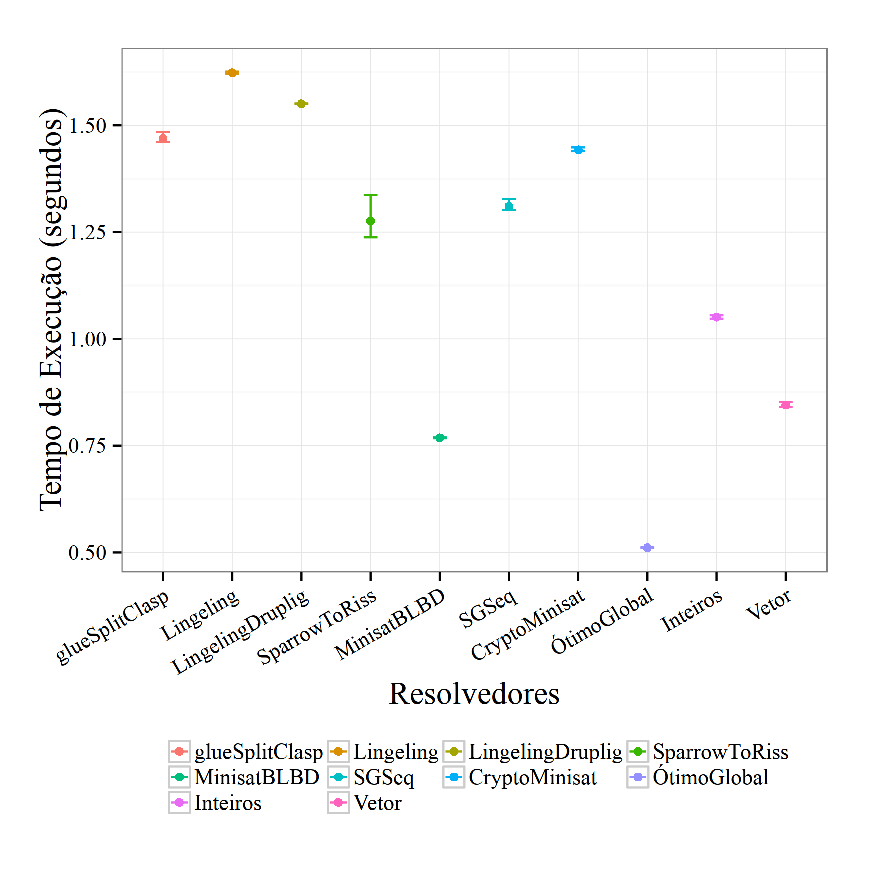
\includegraphics[width=0.5\textwidth]{brute_tuned.eps}
    \captionsetup{width=0.6\textwidth}
    \caption{Desempenho dos Resolvedores, Combinações e Solução Ótima.
             (Média de 30 amostras, as barras de erro representam
             os intervalos de confiança)}
    \label{fig:cmp_brute_tuned}
\end{figure}

Cada ponto na Figura \ref{fig:cmp_brute_tuned} representa a média de 30
execuções do resolvedor correspondente. As barras de erro representam
o intervalo de confiança, calculado através da função \texttt{smean.cl.boot()}
do pacote para a linguagem R \texttt{Hmisc}, que não assume uma distribuição
normal para os valores das amostras.

A solução ótima para o conjunto foi encontrada através de um algoritmo de busca
exaustiva, que executa todos os resolvedores em todas as instâncias e escolhe
o resolvedor com menor média de tempos de execução para cada instância, em 30
execuções.

A busca exaustiva leva cerca de 840 segundos, e os resolvedores
\textit{Inteiros} e \textit{Vetor} representam as soluções encontradas pelo
\emph{auto-tuner} nesse mesmo tempo.

O resolvedor \textit{Inteiros} é a
combinação encontrada pelo \emph{auto-tuner} quando o problema foi codificado
como um conjunto de 100 inteiros. O resolvedor \textit{Vetor} é a combinação
encontrada quando o problema foi codificado como um vetor de inteiros. A
diferença na codificação permite ao \emph{OpenTuner} aplicar diferentes
heurísticas de otimização, e é possível ver que o \emph{auto-tuner}
implementado encontrou uma solução melhor para a codificação em vetor.

Apesar dessa diferença, o \emph{auto-tuner} não encontrou soluções
próximas à ótima no mesmo intervalo de tempo tomado pela busca exaustiva.
Assim, constatamos que existem possibilidades para o aprimoramento do conjunto
de técnicas de busca utilizado pelo \emph{OpenTuner}, para este tipo 
de problema.

\section{Metodologia} \label{sec:met}

Primeiro, será feito um levantamento bibliográfico e um estudo da literatura
relacionada à área de otimização automática utilizando, entre outros, o método
para leitura de trabalhos apresentado por \citet{keshav2007howtoread}.
Concomitantemente, serão  estudadas a fundo a implementação e a arquitetura dos
sistemas OpenTuner, PetaBricks e AMF, para facilitar a especificação das
funcionalidades, classes e estruturas que deverão ser implementadas durante
processo de desenvolvimento.

Depois, será iniciado o ciclo de desenvolvimento das estruturas especificadas
para a implementação dos objetivos, que compreende a implementação,
testes de funcionalidades, testes de desempenho e correções de erros.
Durante a fase de desenvolvimento, serão utilizadas algumas das estratégias
empregadas por metodologias ágeis (\citet{beck2000extreme}), como o
desenvolvimento através de iterações, com prévia avaliação da dificuldade e
distribuição das tarefas.

Os testes de desempenho consistirão na obtenção de dados empíricos para o tempo
de otimização das soluções de problemas computacionalmente difíceis e para o
tempo de execução dessas soluções já otimizadas. Um conjunto de instâncias de
problemas computacionalmente difíceis será escolhido para compor
um \emph{benchmark} de testes de desempenho e devem incluir, entre outros,
instâncias do problema do \emph{bin packing} (\citet{de1981bin}) e do problema
de satisfazibilidade booleana (semelhantes aos experimentos realizados em
\citet{goldman2011optimizing}), problemas já utilizados na avaliação de
desempenho dos sistema PetaBricks e AMF, respectivamente.

Também serão selecionados problemas de otimização para compor um
\emph{benchmark}, como por exemplo a seleção de \emph{flags} de compilação para
GPU --- um problema já estudado por outros pesquisadores do Grupo de Sistemas
de Software da USP (\citet{marcosFAPESP}). Os testes de desempenho serão
realizados em diversas arquiteturas \emph{multi-core} e heterogêneas. Os
resultados das pesquisas e implementações das estratégias do AMF serão
comparados com outros sistemas para \emph{auto-tuning} em diferentes domínios.

As contribuições das estratégias implementadas serão validadas através da
diminuição do tempo de otimização e do tempo de execução das soluções
encontradas. A análise dos resultados será feita através da aplicação do
\emph{benchmark} descrito nesta Seção, que conterá problemas em alguns dos
diversos domínios abordados pelos sistemas descritos na Seção
\ref{sec:trabrel}, e por outros sistemas de referência que serão encontrados
durante a pesquisa. É importante ressaltar que não existem ainda na literatura
sistemas para \emph{auto-tuning} voltados especificamente aos domínios de
problemas computacionalmente difíceis e de decisão.

\section{Cronograma} \label{sec:sched}

A figura \ref{fig:sched} apresenta o cronograma das atividades que serão
desenvolvidas durante o projeto.
No primeiro ano serão realizados estudos da literatura relacionada ao projeto,
visando manter os objetivos orientados aos desenvolvimentos na área e
estudar novos sistemas. Ainda no primeiro ano, serão estudadas a fundo as
implementações dos sistemas PetaBricks, AMF e OpenTuner. O objetivo desse
estudo é analisar e propor possibilidades de aplicação do algoritmo
\emph{portfolio} e da solução do dRSSP na solução do problema do
\emph{auto-tuning}. Inicialmente, serão estudadas as possibilidades de aplicação
da estratégia do AMF para o cálculo de distribuições de recursos computacionais
entre diferentes heurísticas em três situações:

\begin{itemize}
    \item Como técnica de \emph{auto-tuning} independente, implementada
        no PetaBricks e OpenTuner, especificamente na solução de problemas
        de decisão computacionalmente difíceis, como por exemplo o problema
        de satisfabilidade booleana.
    \item Como metatécnica para seleção de métodos de busca no OpenTuner;
    \item Como seletora de operadores de mutação do algoritmo genético
        utilizado no PetaBricks, em comparação com o MAB AUC.
\end{itemize}

No segundo ano serão implementadas as possibilidades estudadas no primeiro ano.
Serão estudadas a adaptação e a utilização do algoritmo \emph{portfolio} na
solução do problema do \emph{auto-tuning online} e no caso não restrito a
problemas de decisão computacionalmente difíceis. Os conhecimentos adquiridos
durante a revisão bibliográfica do primeiro ano permitirão realizar no segundo
ano uma busca na literatura por possíveis outros sistemas de referência para o
projeto. Durante a duração do programa de Doutorado Direto e passado o tempo
mínimo de matrícula exigido pela FAPESP, submeteremos um projeto de pesquisa
para estágio no exterior através do programa BEPE.

No terceiro e quarto anos do programa de Doutorado Direto continuarão sendo
implementadas as técnicas estudadas nos anos anteriores. Serão implementadas
soluções para o problema do \emph{auto-tuning online} e de problemas de
otimização baseadas no algoritmo \emph{portfolio}. O cronograma menos detalhado
para esses dois anos resulta das atividades planejadas para esse período serem
fortemente dependentes dos resultados dos anos anteriores.

Serão realizadas comparações entre todas as implementações, através da análise
de seu tempo de otimização e desempenho. Utilizaremos, a princípio, os
\emph{benchmarks} dos sistemas PetaBricks e OpenTuner e o \emph{benchmark} para
problemas computacionalmente difíceis, que será elaborado como descrito na
seção \ref{sec:met}. Os testes e estudos de desempenho das implementações
também serão realizados em diferentes arquiteturas computacionais, como por
exemplo arquiteturas heterogêneas e \emph{multi-core}.

Finalmente, serão feitas implementações de abstrações de alto
nível, que deverão encapsular as implementações dos conceitos estudados
anteriormente. Essas abstrações devem facilitar a uso das implementações
realizadas como biblioteca e podem tomar a forma de um arcabouço para o
\emph{auto-tuning online} de programas.

\subsubsection{Sobre o Candidato}

O candidato à Bolsa de Doutorado Direto formou-se em 2014 no Curso de Ciências
Moleculares da Universidade de São Paulo, com boa média e sem reprovações em
disciplinas. Durante os dois anos finais da graduação, realizou Iniciação
Científica em Sistemas Multiagentes e Computação Musical no Instituto de
Matemática e Estatística da USP, com apoio do CNPq.

Também em 2014, o candidato publicou o trabalho realizado durante a graduação
(\citet{bruel2014protocol}) na principal conferência da área, a
\emph{40th International Computer Music Conference (ICMC) joint with the
11th Sound \& Music Computing conference (SMC)}.

\begin{figure}[H]
    \centering
\begin{center}
    \begin{tabular}{ | >{\centering\arraybackslash}p{3.25cm} |
    >{\centering\arraybackslash}p{3.25cm} |
    >{\centering\arraybackslash}p{3.25cm} |
    >{\centering\arraybackslash}p{3.25cm} |}
    \multicolumn{4}{c}{} \\
    \hline
    1º Ano & 2º Ano & 3º Ano & 4º Ano \\ \hline
    \cellcolor{gray!96} Estudo das Possibilidades das Técnicas do AMF  & \cellcolor{gray!14} Estudo do algoritmo \emph{portfolio} no \emph{auto-tuning online} & \multicolumn{2}{p{7cm}|}{\cellcolor{gray!96} Implementação do algoritmo \emph{portfolio} no contexto do \emph{auto-tuning online} e de problemas de otimização} \\
    \cellcolor{gray!84} Estudo da Implementação do PetaBricks & \cellcolor{gray!28} Implementação das possibilidades estudadas & \multicolumn{2}{p{7cm}|}{\cellcolor{gray!70} Implementação de abstrações alto nível para as implementações já realizadas} \\
    \cellcolor{gray!70} Estudo da Implementação do AMF & \cellcolor{gray!42} Busca por novos sistemas de referência & \multicolumn{2}{p{7cm}|}{\cellcolor{gray!56} Aplicação de benchmarks e testes de desempenho em diferentes arquiteturas} \\
    \cellcolor{gray!56} Estudo da Implementação do OpenTuner & \cellcolor{gray!70} Estudo do algoritmo \emph{portfolio} no \emph{auto-tuning} de problemas de otimização & \multicolumn{2}{l|}{} \\
    \cellcolor{gray!42} Revisão Bibliográfica &  \cellcolor{gray!84} Submissão de proposta ao BEPE & \multicolumn{2}{l|}{} \\
    \cellcolor{gray!28} 2 disciplinas do programa por semestre &  \cellcolor{gray!96} 2 disciplinas do programa por semestre & \multicolumn{2}{l|}{} \\
    \cellcolor{gray!14} Escolha de Benchmarks de Referência & \multicolumn{3}{l|}{} \\
    \hline
    \end{tabular}
\end{center}
    \caption{Cronograma para as atividades do projeto.}
    \label{fig:sched}
\end{figure}

\newpage
\bibliographystyle{plainnat}
\bibliography{projeto}

\end{document}
